\documentclass[12pt,technote,a4paper,onecolumn]{IEEEtran}
\usepackage[left=2cm,right=2cm,top=2cm,bottom=2cm]{geometry}
\usepackage[utf8]{inputenc}
\usepackage[english]{babel}


%\usepackage{biblatex}
\usepackage{cite}

\usepackage{amsmath}
\usepackage{amsfonts}
\usepackage{amssymb}
\usepackage{graphicx}
\usepackage[colorlinks=false,linktoc=page,linkcolor=blue]{hyperref}
\usepackage{textcomp}
\usepackage{xcolor}
\usepackage{algorithmic}
\usepackage{circuitikz}
\usepackage{tikz}
\usetikzlibrary{decorations.markings}
\newif\iflabrev
\usepackage{blox}


\title{EC601: Assignment 1}
\author{	\IEEEauthorblockN{Dhiman Sarkar}
			\IEEEauthorblockA{\\
							Roll: 19101105086\\
							Department of Electronics and Communication Engineering\\
							Jalpaiguri Government Engineering College\\
							Email: ds2286@ece.jgec.ac.in
							}
		}

\begin{document}
\maketitle

\tableofcontents


\newpage
\section{Problem 1}
1) Consider the system defined by
\begin{equation}
	\begin{bmatrix}
		\dot{x_1} \cr \dot{x_2} \cr \dot{x_3}
	\end{bmatrix} =
	\begin{bmatrix}
		0 & 1 & 0 \\
		0 & 0 & 1 \\
		-6 & -11 &  -6
	\end{bmatrix}
	\begin{bmatrix}
		x_1 \cr x_2 \cr x_3
	\end{bmatrix} +
	\begin{bmatrix}
	0 \cr 0 \cr 1
	\end{bmatrix} u			\nonumber
\end{equation}
Except for an obvious choice of $c_1=c_2=c_3=0$, find an example of a set of $c_1$, $c_2$, $c_3$ that will make the system unobservable.

\vspace{10pt}
$\blacksquare$\\


Lets say, $ y = C \cdot x$ where, $C = \left[c_1~c_2~c_3\right]$\\
We have $A = $
	$\begin{bmatrix}
		0 & 1 & 0 \\
		0 & 0 & 1 \\
		-6 & -11 &  -6
	\end{bmatrix}$
	
\begin{eqnarray} % CA
\therefore	CA &=& 
	\begin{bmatrix}
		c_1 & c_2 & c_3
	\end{bmatrix}
	\begin{bmatrix}
		0 & 1 & 0 \\
		0 & 0 & 1 \\
		-6 & -11 &  -6
	\end{bmatrix} \nonumber\\
	&=&\begin{bmatrix}
	-6c_3 & c_1 - 11 c_3 & c_2 - 6 c_3
	\end{bmatrix}
\end{eqnarray}

\begin{eqnarray} %CA^2
\therefore CA^2 &=&
	\begin{bmatrix}
	-6c_3 & c_1 - 11 c_3 & c_2 - 6 c_3
	\end{bmatrix}
	\cdot
	\begin{bmatrix}
		0 & 1 & 0 \\
		0 & 0 & 1 \\
		-6 & -11 &  -6
	\end{bmatrix} \nonumber\\
	&=& \begin{bmatrix}
	-6 c_2 + 36 c_3 & -11 c_2 + 60 c_3 & c_1 - 6 c_2 + 25 c_3 
	\end{bmatrix}
\end{eqnarray}

\begin{eqnarray} %Q_O
\therefore \text{Observability Matrix, }  Q_O &=&
	\begin{bmatrix}
	A\\CA\\CA^2
	\end{bmatrix} \nonumber\\
	&=& \begin{bmatrix}
		c_1 & c_2 & c_3\\
		-6c_3 & c_1 - 11 c_3 & c_2 - 6 c_3\\
		-6 c_2 + 36 c_3 & -11 c_2 + 60 c_3 & c_1 - 6 c_2 + 25 c_3
	\end{bmatrix}\\
\end{eqnarray}

\begin{eqnarray}
\therefore |Q_O| &=&
	\left| \begin{matrix}
		c_1 & c_2 & c_3\\
		-6c_3 & c_1 - 11 c_3 & c_2 - 6 c_3\\
		-6 c_2 + 36 c_3 & -11 c_2 + 60 c_3 & c_1 - 6 c_2 + 25 c_3
	\end{matrix} \right| \\ 
	&=& 6c_3 ((c_2 (c_1 - 6 c_2 + 25 c_3c_1 - 6 c_2 + 25 c_3) - c_3(-11 c_2 + 60 c_3)) \nonumber\\
	&&+( c_1 - 11 c_3)(c_1(c_1 - 6 c_2 + 25 c_3c_1 - 6 c_2 + 25 c_3) - c_3 (-6 c_2 + 36 c_3)) \nonumber\\
	&&-(c_2 - 6 c_3)(c_1(-11 c_2 + 60 c_3 ) - c_2(-6 c_2 + 36 c_3)) \label{eq:1}\\
	&=& c_1^3 - 6 c_2 c_1^2 + 14 c_3 c_1^2 + 11 c_2^2 c_1 + 49 c_3^2 c_1 \nonumber\\
	&&- 48 c_2 c_3 c_1 - 6 c_2^3 + 36 c_3^3 - 66 c_2 c_3^2 + 36 c_2^2 c_3 \text{~\cite{det1}}
\end{eqnarray}

The question asked to find the non-trivial solutions of $c_1, c_2, c_3$ (i.e. $c_1\neq c_2\neq c_3 \neq 0$) such that the system is unobservable (i.e. $|Q_O|=0$)

$\therefore$ to eliminate the trivial solutions, the following relations are chosen : $|Q_O|=0$

from the first, second and third part of Eq.\ref{eq:1} we get respectively,
\begin{eqnarray}
&(c_2 (c_1 - 6 c_2 + 25 c_3c_1 - 6 c_2 + 25 c_3) - c_3(-11 c_2 + 60 c_3) = 0 \label{eq:2} \\
&( c_1 - 11 c_3) =0 \label{eq:3}\\
&(c_2 - 6 c_3) = 0 \label{eq:4} 
\end{eqnarray}
Now solving Eq.\ref{eq:2}, Eq.\ref{eq:3}, Eq.\ref{eq:4} we get,\\
\begin{eqnarray}
c_1 = \frac{7}{5} ~,~ c_2 = \frac{42}{55} ~,~ c_3 = \frac{7}{55} \nonumber \text{\cite{detsol1}}
\end{eqnarray}

\hfill$\blacksquare$
\newpage

\section{Problem 2}
2) Obtain the transfer function $\frac{e_i}{e_o}$ of the electrical circuit shown in the figure.\\

\begin{center}
\begin{circuitikz}
\draw (0,0) to[open, l=$e_i$] (0,3);
\draw (0,0) to[short, o-*] (3,0) to[american inductor, l_=$L$, mirror] (3,3) node[label={[color=blue]$V_L$}]{} to[american resistor, l_=$R_1$, f<=$i_1$, *-*] (0,3) to[short, *-o] (0,3);
\draw (3,0) -- (6,0) to[capacitor, l_=$C$] (6,3) to[R, l_=$R_2$, f<=$i_2$] (3,3);
\draw (6,0) to[short, *-o] (7,0);
\draw (6,3) to[short, *-o] (7,3);
\draw (7,0) to[open, l_=$e_o$] (7,3);
\draw [->,shift={(1.5,1.5)}] (120:.7cm) arc (120:-90:.7cm) node at(0,0){$i_1$};
\draw [->,shift={(4.5,1.5)}] (120:.7cm) arc (120:-90:.7cm) node at(0,0){$i_2$};
\end{circuitikz}\end{center}


$\blacksquare$
Lets say the node voltage of L is $V_L$
\begin{equation}
\therefore V_L = e_i \times \frac{G_1}{G_1+Y_2}
\end{equation}
Where, 
\begin{eqnarray}
&G_1 &=\frac{1}{R_1} \nonumber \\
&Y_2 &=\frac{1}{sL}+\frac{1}{R_2+\frac{1}{sC}} \nonumber
\end{eqnarray}
\begin{eqnarray}
\therefore e_o &= &V_L \times \frac{\frac{1}{sC}}{R_2+\frac{1}{sC}}\\
\implies e_o &= &e_i \times \frac{G_1}{G_1+Y_2} \times \frac{\frac{1}{sC}}{R_2+\frac{1}{sC}} \nonumber\\
\implies \frac{e_o}{e_i} &= &H(s) = \frac{G_1}{G_1+Y_2} \times \frac{\frac{1}{sC}}{R_2+\frac{1}{sC}} \nonumber\\
\implies H(s) &= &\frac{\frac{1}{R_1}}{\frac{1}{R_1}+\frac{1}{sL}+\frac{1}{R_2+\frac{1}{sC}}} \times \frac{\frac{1}{sC}}{R_2+\frac{1}{sC}} \nonumber\\
\implies H(s) &= &\frac{sL}{LC(R_1+R_2)s^2 + (R_1 R_2 C+L) s + R_1}
\end{eqnarray}\\


\hfill $\blacksquare$
\newpage


\section{Problem 3}
3) Simplify the block diagram shown in Figure. Then obtain the closed-loop transfer function $\frac{C(s)}{R(s)}$.


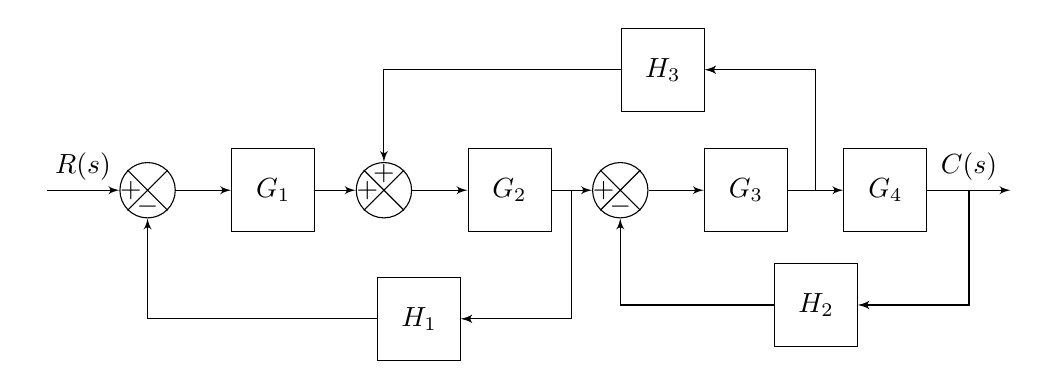
\begin{tikzpicture}
	\bXInput{A}
	\bXComp{B}{A} \bXLink[$R(s)$]{A}{B}
	\bXBloc{C}{$G_1$}{B} \bXLink{B}{C}
	\bXSuma{D}{C} \bXLink{C}{D}
	\bXBloc{E}{$G_2$}{D} \bXLink{D}{E}
	\bXComp{F}{E} \bXLink{E}{F}
	\bXBloc{G}{$G_3$}{F} \bXLink{F}{G}
	\bXBloc{H}{$G_4$}{G} \bXLink{G}{H}
	\bXOutput[3]{I}{H} \bXLink[$C(s)$]{H}{I}
	
	%Feedback Paths
	\bXBranchy{H-I}{J}
	\bXChainReturn{J}{a/$H_2$} \bXLinkyx{H-I}{a} \bXLinkxy{a}{F}

	\bXBranchy[-4]{G-H}{K}
	\bXChainReturn{K}{b/$H_3$} \bXLinkyx{G-H}{b} \bXLinkxy{b}{D}
	
	\bXBranchy{E-F}{L}
	\bXChainReturn{L}{c/$H_1$} \bXLinkyx{E-F}{c} \bXLinkxy{c}{B}
\end{tikzpicture}

\vspace{10pt}
$\blacksquare$

Step 1:\\
	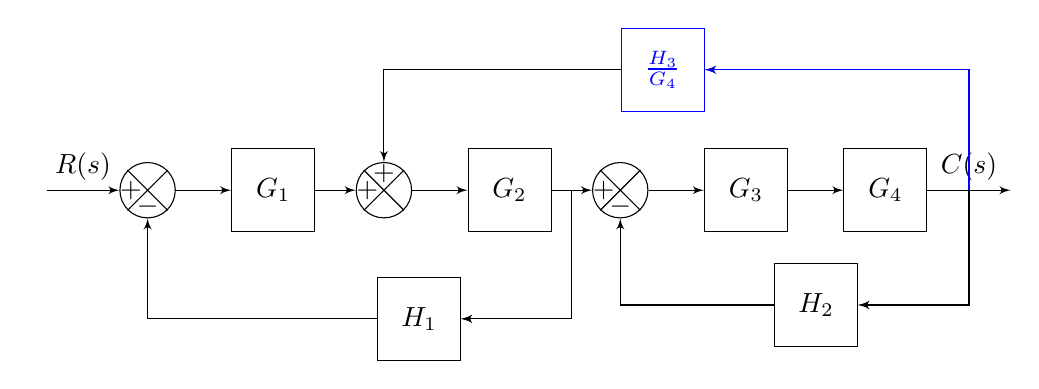
\begin{tikzpicture}
	\bXInput{A}
	\bXComp{B}{A} \bXLink[$R(s)$]{A}{B}
	\bXBloc{C}{$G_1$}{B} \bXLink{B}{C}
	\bXSuma{D}{C} \bXLink{C}{D}
	\bXBloc{E}{$G_2$}{D} \bXLink{D}{E}
	\bXComp{F}{E} \bXLink{E}{F}
	\bXBloc{G}{$G_3$}{F} \bXLink{F}{G}
	\bXBloc{H}{$G_4$}{G} \bXLink{G}{H}
	\bXOutput[3]{I}{H} \bXLink[$C(s)$]{H}{I}
	
	%Feedback Paths
	\bXBranchy{H-I}{J}
	\bXChainReturn{J}{a/$H_2$} \bXLinkyx{H-I}{a} \bXLinkxy{a}{F}

	\bXBranchy[-4]{G-H}{K}
	\bXStyleBloc{blue} \bXChainReturn{K}{b/$\frac{H_3}{G_4}$} \bXLineStyle{blue} \bXLinkyx{H-I}{b} \bXDefaultLineStyle\bXLinkxy{b}{D}\bXStyleBlocDefault
	
	\bXBranchy{E-F}{L}
	\bXChainReturn{L}{c/$H_1$} \bXLinkyx{E-F}{c} \bXLinkxy{c}{B}
	\end{tikzpicture}
	
Step 2:\\
	\begin{tikzpicture}
	\bXInput{A}
	\bXComp{B}{A} \bXLink[$R(s)$]{A}{B}
	\bXBloc{C}{$G_1$}{B} \bXLink{B}{C}
	\bXSuma{D}{C} \bXLink{C}{D}
	\bXBloc{E}{$G_2$}{D} \bXLink{D}{E}
	\bXComp{F}{E} \bXLink{E}{F}
	\bXStyleBloc{blue} \bXBloc{H}{$G_3G_4$}{G} \bXLink{F}{H} \bXStyleBlocDefault
	\bXOutput[3]{I}{H} \bXLink[$C(s)$]{H}{I}
	
	%Feedback Paths
	\bXBranchy{H-I}{J}
	\bXChainReturn{J}{a/$H_2$} \bXLinkyx{H-I}{a} \bXLinkxy{a}{F}

	\bXBranchy[-4]{G-H}{K}
	\bXChainReturn{K}{b/$\frac{H_3}{G_4}$} \bXLinkyx{H-I}{b} \bXLinkxy{b}{D}\bXStyleBlocDefault
	
	\bXBranchy{E-F}{L}
	\bXChainReturn{L}{c/$H_1$} \bXLinkyx{E-F}{c} \bXLinkxy{c}{B}
	\end{tikzpicture}
	
Step 3:\\
	\begin{tikzpicture}
	\bXInput{A}
	\bXComp{B}{A} \bXLink[$R(s)$]{A}{B}
	\bXBloc{C}{$G_1$}{B} \bXLink{B}{C}
	\bXSuma{D}{C} \bXLink{C}{D}
	\bXBloc{E}{$G_2$}{D} \bXLink{D}{E}
	\bXStyleBloc{blue} \bXBloc{H}{$\frac{G_3G_4}{1+G_3G_4H_2}$}{E} \bXLink{E}{H} \bXStyleBlocDefault
	\bXOutput[3]{I}{H} \bXLink[$C(s)$]{H}{I}
	
	%Feedback Paths

	\bXBranchy[-4]{H-I}{K}
	\bXChainReturn{K}{b/$\frac{H_3}{G_4}$} \bXLinkyx{H-I}{b} \bXLinkxy{b}{D}\bXStyleBlocDefault
	
	\bXBranchy{E-F}{L}
	\bXChainReturn{L}{c/$H_1$} \bXLinkyx{E-F}{c} \bXLinkxy{c}{B}
	\end{tikzpicture}


Step 4:\\
	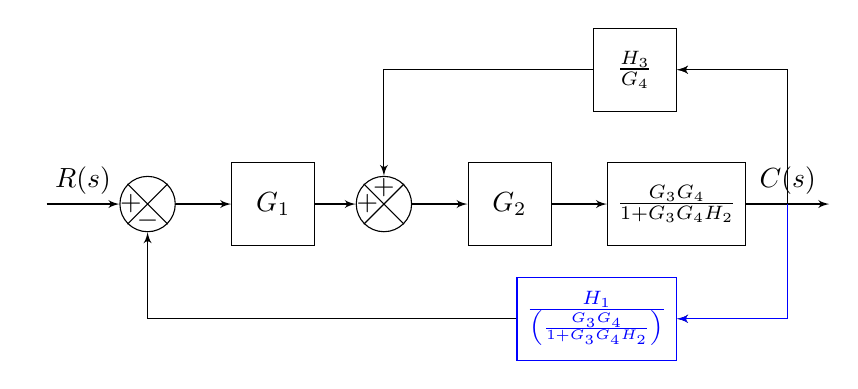
\begin{tikzpicture}
	\bXInput{A}
	\bXComp{B}{A} \bXLink[$R(s)$]{A}{B}
	\bXBloc{C}{$G_1$}{B} \bXLink{B}{C}
	\bXSuma{D}{C} \bXLink{C}{D}
	\bXBloc{E}{$G_2$}{D} \bXLink{D}{E}
	\bXBloc{H}{$\frac{G_3G_4}{1+G_3G_4H_2}$}{E} \bXLink{E}{H} 
	\bXOutput[3]{I}{H} \bXLink[$C(s)$]{H}{I}
	
	%Feedback Paths

	\bXBranchy[-4]{H-I}{K}
	\bXChainReturn{K}{b/$\frac{H_3}{G_4}$} \bXLinkyx{H-I}{b} \bXLinkxy{b}{D}\bXStyleBlocDefault
	
	\bXBranchy{H-I}{L}
	\bXStyleBloc{blue} \bXChainReturn{L}{c/$\frac{H_1}{\left(\frac{G_3G_4}{1+G_3G_4H_2}\right)}$} \bXStyleBlocDefault \bXLineStyle{blue} \bXLinkyx{H-I}{c} \bXDefaultLineStyle \bXLinkxy{c}{B} 
	\end{tikzpicture}
	
	
Step 5:\\
	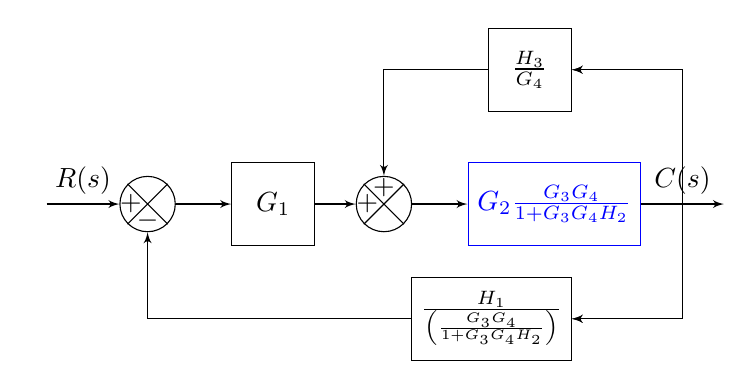
\begin{tikzpicture}
	\bXInput{A}
	\bXComp{B}{A} \bXLink[$R(s)$]{A}{B}
	\bXBloc{C}{$G_1$}{B} \bXLink{B}{C}
	\bXSuma{D}{C} \bXLink{C}{D}
	 \bXStyleBloc{blue} \bXBloc{H}{$G_2\frac{G_3G_4}{1+G_3G_4H_2}$}{D} \bXLink{D}{H}  \bXStyleBlocDefault
	\bXOutput[3]{I}{H} \bXLink[$C(s)$]{H}{I}
	
	%Feedback Paths

	\bXBranchy[-4]{H-I}{K}
	\bXChainReturn{K}{b/$\frac{H_3}{G_4}$} \bXLinkyx{H-I}{b} \bXLinkxy{b}{D}\bXStyleBlocDefault
	
	\bXBranchy{H-I}{L}
	\bXChainReturn{L}{c/$\frac{H_1}{\left(\frac{G_3G_4}{1+G_3G_4H_2}\right)}$} \bXLinkyx{H-I}{c} \bXLinkxy{c}{B} 
	\end{tikzpicture}


Step 6:\\
	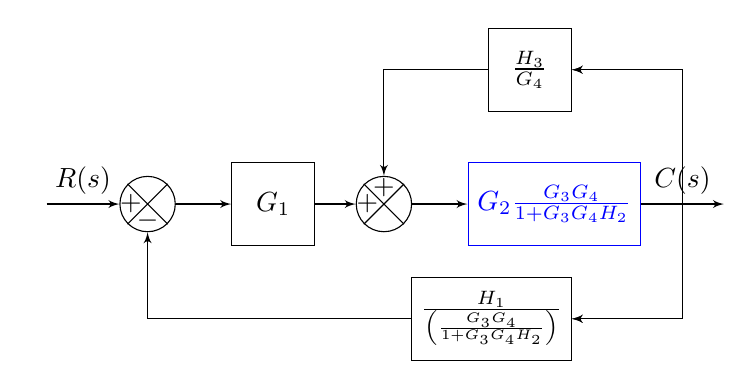
\begin{tikzpicture}
	\bXInput{A}
	\bXComp{B}{A} \bXLink[$R(s)$]{A}{B}
	\bXBloc{C}{$G_1$}{B} \bXLink{B}{C}
	\bXSuma{D}{C} \bXLink{C}{D}
	 \bXStyleBloc{blue} \bXBloc{H}{$G_2\frac{G_3G_4}{1+G_3G_4H_2}$}{D} \bXLink{D}{H}  \bXStyleBlocDefault
	\bXOutput[3]{I}{H} \bXLink[$C(s)$]{H}{I}
	
	%Feedback Paths

	\bXBranchy[-4]{H-I}{K}
	\bXChainReturn{K}{b/$\frac{H_3}{G_4}$} \bXLinkyx{H-I}{b} \bXLinkxy{b}{D}\bXStyleBlocDefault
	
	\bXBranchy{H-I}{L}
	\bXChainReturn{L}{c/$\frac{H_1}{\left(\frac{G_3G_4}{1+G_3G_4H_2}\right)}$} \bXLinkyx{H-I}{c} \bXLinkxy{c}{B} 
	\end{tikzpicture}
	
	
Step 7:\\
	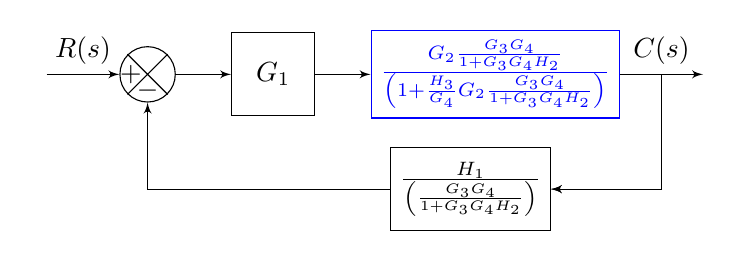
\begin{tikzpicture}
	\bXInput{A}
	\bXComp{B}{A} \bXLink[$R(s)$]{A}{B}
	\bXBloc{C}{$G_1$}{B} \bXLink{B}{C}
	\bXStyleBloc{blue} \bXBloc{H}{$\frac{G_2\frac{G_3G_4}{1+G_3G_4H_2}}{\left( 1+\frac{H_3}{G_4}G_2\frac{G_3G_4}{1+G_3G_4H_2} \right)}$}{C} \bXLink{C}{H}  \bXStyleBlocDefault
	\bXOutput[3]{I}{H} \bXLink[$C(s)$]{H}{I}
	
	%Feedback Paths
	\bXBranchy{H-I}{L}
	\bXChainReturn{L}{c/$\frac{H_1}{\left(\frac{G_3G_4}{1+G_3G_4H_2}\right)}$} \bXLinkyx{H-I}{c} \bXLinkxy{c}{B} 
	\end{tikzpicture}
	
	
Step 8:\\
	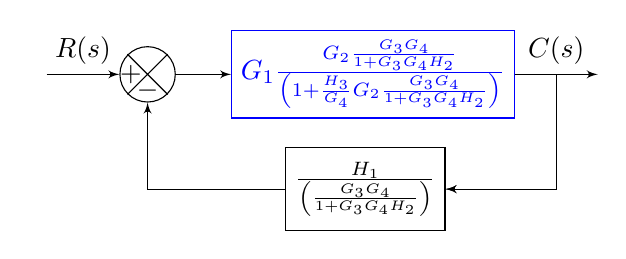
\begin{tikzpicture}
	\bXInput{A}
	\bXComp{B}{A} \bXLink[$R(s)$]{A}{B}
	\bXStyleBloc{blue} \bXBloc{H}{$G_1\frac{G_2\frac{G_3G_4}{1+G_3G_4H_2}}{\left( 1+\frac{H_3}{G_4}G_2\frac{G_3G_4}{1+G_3G_4H_2} \right)}$}{B} \bXLink{B}{H}  \bXStyleBlocDefault
	\bXOutput[3]{I}{H} \bXLink[$C(s)$]{H}{I}
	
	%Feedback Paths
	\bXBranchy{H-I}{L}
	\bXChainReturn{L}{c/$\frac{H_1}{\left(\frac{G_3G_4}{1+G_3G_4H_2}\right)}$} \bXLinkyx{H-I}{c} \bXLinkxy{c}{B} 
	\end{tikzpicture}
	

Step 9:\\
	
	\def \G {G_1\frac{G_2\frac{G_3G_4}{1+G_3G_4H_2}}{\left( 1+\frac{H_3}{G_4}G_2\frac{G_3G_4}{1+G_3G_4H_2} \right)}}
	\def \H {\frac{H_1}{\left(\frac{G_3G_4}{1+G_3G_4H_2}\right)}}

	\begin{tikzpicture}\begin{Large}

	\bXInput{A} 
	\bXLink[$R(s)$]{A}{H}
	\bXStyleBloc{blue} \bXBloc{H}{\Huge $ \frac{\G}{\left( 1+ \left(\G\right) \left(\H\right) \right)} $}{B}  \bXStyleBlocDefault
	\bXOutput[3]{I}{H} \bXLink[$C(s)$]{H}{I}
	
	%Feedback Paths
	\end{Large}	
	\end{tikzpicture}

\begin{eqnarray}
\therefore \text{Transfer Function} \frac{C(s)}{R(s)} =&& \frac{\G}{\left( 1+ \left(\G\right) \left(\H\right) \right)}\\
=&& 
\end{eqnarray}

% \bXStyleBloc{blue} \bXStyleBlocDefault
% \bXLineStyle{blue} \bXDefaultLineStyle

\hfill $\blacksquare$
\newpage



\section{Problem 4}
4) Draw the signal low graph of the following electrical circuit and find its transfer function using Mason’s gain formula.\\
\begin{center}
\begin{circuitikz}[american]
	\draw (0,0) to[short, -*] (3,0) to[R, l_=$R_3$] (3,3) to[R,*-, l_=$R_1$] (0,3) to [V, l_=$v_1$] (0,0);
	\draw [->,shift={(1.5,1.5)}] (150:.7cm) arc (150:30:.7cm) node at(0,0){$i_1$};
	\draw (3,0) to[short, *-*] (6,0) to[R, l_=$R_4$, *-*] (6,3) to[R,l=$R_2$, *-*] (3,3);
	\draw [->,shift={(4.5,1.5)}] (150:.7cm) arc (150:30:.7cm) node at(0,0){$i_2$};
	\draw (3,3) to[short] (3,5) to[I, l=$\alpha i_1$] (6,5) to[short] (6,3);
	\draw [->,shift={(4.5,3.5)}] (150:.7cm) arc (150:30:.7cm) node at(0,0){$\alpha i_1$};
	\draw (6,0) to[short, *-o] (8,0) to[open,l_=$v_3$] (8,3) to[short, o-*] (6,3);
	
	%Custom Nodes
	\draw (3.2,3.2) node[blue]{$v_2$}; 
	\draw (0.2,3.2) node[blue]{$v_1$}; 
	\draw (6.2,3.2) node[blue]{$v_3$};
\end{circuitikz}
\end{center}

$\blacksquare$

Custom Nodes has been marked in {\color{blue} blue}.

\begin{eqnarray}
	v_1 &=& \text{Input Voltage}\\
	v_2 &=&(i_1 - i_2)(R_3) \nonumber\\
		&=& \left(R_3\right)i_1 + \left(-R_3\right)i_2\\
	v_3 &=& (\alpha i_1 + i_2)R_4 \nonumber\\
		&=& (\alpha R_4)i_1 + (R_4)i_2\\
	i_1 &=& \frac{v_1-v_2}{R_1} \nonumber\\
		&=& \left( \frac{1}{R_1} \right)v_1 + \left( -\frac{1}{R_1} \right)v_2\\
	i_2 &=& \frac{v_2-v_3}{R_2} \nonumber\\
		&=& \left( \frac{1}{R_2}  \right)v_2 + \left( -\frac{1}{R_2} \right)v_3
\end{eqnarray}

Signal Flow Graph of the given circuit:\\
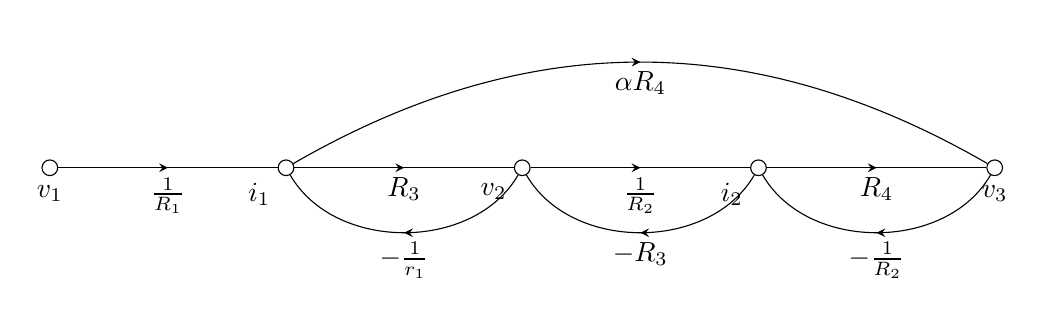
\begin{tikzpicture}
[
label revd/.is if=labrev,
%label revd/.default=true,
amark/.style={
            decoration={             
                        markings,   
                        mark=at position {0.5} with { 
                                    \arrow{stealth},
                                    \iflabrev \node[above] {#1};\else \node[below] {#1};\fi
                        }
            },
            postaction={decorate}
},
terminal/.style 2 args={draw,circle,inner sep=2pt,label={#1:#2}},
]

%Place the nodes
\node[terminal={below}{$v_1$}] (a) at (0,0) {};	 		%v1 = a
\node[terminal={below left}{$i_1$}] (b) at (3,0) {}; 	%i1 = b
\node[terminal={below left}{$v_2$}] (c) at (6,0) {}; 	%v2 = c
\node[terminal={below left}{$i_2$}] (d) at (9,0) {}; 	%i2 = d
\node[terminal={below}{$v_3$}] (e) at (12,0) {}; 		%v3 = e

%connections
%node v2 = c
\draw[amark=$R_3$] (b) to (c);
\draw[amark=$-R_3$] (d) to[bend left = 60] (c);
%node v3 = e
\draw[amark=$\alpha R_4$] (b) to[bend left=30] (e);
\draw[amark=$R_4$] (d) to (e);
%node i1 = b
\draw[amark=$\frac{1}{R_1}$] (a) to (b);
\draw[amark=$-\frac{1}{r_1}$] (c) to[bend left=60] (b);
%node i2 = d
\draw[amark=$\frac{1}{R_2}$] (c) to (d); 
\draw[amark=$-\frac{1}{R_2}$] (e) to[bend left=60] (d);
\end{tikzpicture}

\hfill $\blacksquare$
\newpage


\bibliography{Reference}
\bibliographystyle{IEEEtran}
\end{document}
